\section{Protokoll för kommunikation}

\subsection{Kommunikation mellan PC och huvudmodul}

Kommunikation mellan PC-enhet och huvudenhet sker via Blåtand. En instruktion ges som en sträng på formen $command1=arg1,...,argN;command2=arg1,...,argN$ med ett godtyckligt antal instruktioner där antalet argument per instruktion specificeras i avsnitt \ref{designspec:protokoll-pc-huvud-kommandon}.

\subsubsection{Instruktioner} \label{designspec:protokoll-pc-huvud-kommandon}

\begin{table}[h]
	\centering
		\begin{tabularx}{\textwidth}{| l | l | X |}
			\hline
			\textbf{Instruktion} & \textbf{Argument} & \textbf{Beskrivning} \\
			\hline
			{motor} & {L,R} & {L och R anger hastigheten på det vänstra, respektive högra hjulparet} \\
			\hline
			{arm} & {X,Y,Z,P,G} & {X,Y,Z är koordinaten i rummet dit armens hand skall röra sig. Armens fundament är origo, P anger handens vinkel i förhållande till Z-axeln och G anger avståndet mellan handens fingrar.} \\
			\hline
			{calibrate} & {} & {Begär kalibrering av robotens sensorer} \\
			\hline
			{status} & {} & {Begär statusrapport från robot} \\
			\hline
			{automotor} & {M} & {Ange om robotens motorer skall styras från PC-enheten (0) eller huvudenheten (1)} \\
			\hline
			{autoarm} & {M} & {Ange om robotarmen skall styras från PC-enheten (0) eller huvudenheten (1)} \\
			\hline
			{start} & {} & {Initiera körning} \\
			\hline
		\end{tabularx}
	\caption{Instruktioner från PC-enhet till huvudenhet} \label{protokoll:pc-huvud}
\end{table}
%\todo{Högre/lägre värden på t.ex X eller P gör vad, precis? X och Y =-+38cm,0<=Z<=46 bestäm upplösning}\\
%\todo{Illustrera koordinatsystem m. bild}
L och R:s begränsningar där 100 representerar maximal hastighet framåt och -100 representerar maximal hastighet bakåt
$$-100\leq L \leq 100$$
$$-100\leq R \leq 100$$
Begränsningar på X,Y,Z motsvarar hur långt roboten kan sträcka sig i varje led
$$-3800\leq X \leq 3800$$
$$-3800\leq Y \leq 3800$$
$$0\leq Z \leq 4600$$
Begränsningarna på G motsvarar servots input för position
$$0\leq G \leq 1024$$
Begränsningarna på P motsvarar vilken vinkel robotens hand kan ha mot XY planet.
$$-90\leq P \leq 90$$

\todo{Bygg om}

\subsection{Kommunikation mellan huvudmodul och sensormodul}
Kommunikation mellan huvudmodul och sensormodul sker via en SPI-buss. Instruktioner från huvudmodulen ges i form av en byte. De fyra första bitarna anger vilken instruktion som skall utföras. De sista fyra anger vilken sensor instruktionen gäller. Tabell \ref{protokoll:huvud-sensor} och \ref{protokoll:huvud-sensor-adress} under avsnitt \ref{designspec:protokoll-huvud-sensor-instr} specificerar de instruktioner som finns respektive vilken adress som avser vilken sensor. \\
Sensorenheten svarar med endast data. En byte per fototransistor i linjesensorn. En byte för vardera avståndssensor. I fallet med instruktionen \textit{läs data från alla sensorer} skickas sensorernas data seriellt i följande ordning: 1. Linjesensor, 2: Avståndssensor Höger, 3: Avståndssensor Vänster.

\subsubsection{Instruktioner} \label{designspec:protokoll-huvud-sensor-instr}

\begin{table}[h]
	\centering
		\begin{tabularx}{\textwidth}{| l | l | X |}
			\hline
			\textbf{Instruktion} & \textbf{Argument} & \textbf{Beskrivning} \\
			\hline
			{0000} & {A} & {Returnera sensordata för A} \\
			\hline
			{0001} & {A} & {Kalibrera sensor A} \\
			\hline
		\end{tabularx}
	\caption{Instruktioner från huvudenhet till sensorenhet} \label{protokoll:huvud-sensor}
\end{table}

\begin{table}[h]
	\centering
		\begin{tabularx}{\textwidth}{| l | X |}
			\hline
			\textbf{Adress} & \textbf{Beskrivning} \\
			\hline
			{0000} & {Linjesensor Fram} \\
			\hline
			{0010} & {Avståndssensor Höger} \\
			\hline
			{0011} & {Avståndssensor Vänster} \\
			\hline
			{1111} & {Adressera samtliga sensorer} \\
			\hline
		\end{tabularx}
	\caption{Adresser för instruktioner till sensorenhet} \label{protokoll:huvud-sensor-adress}
\end{table}

\subsection{Kommunikation mellan huvudenhet och styrenhet} \label{protokoll:pc-motor}
Kommunikation mellan huvudmodul och motormodul sker via en SPI-buss. Det finns en busy-flagga kopplad till huvudmodulen som går låg när armen är i rörelse. \\
En instruktion består av tre bytes. Den första byten innehåller instruktionen och vilket servo eller vilken motor som avses. De första fyra bitarna av denna byte definierar vilket kommando som skall utföras. De nästkommande fyra vilken enhet det skall utföras av. Tabell \ref{protokoll:pc-motor-tabell} och \ref{protokoll:pc-motor-adress-tabell} i avsnitt \ref{designspec:protokoll-pc-motor-instr} specificerar de instruktioner som finns och vilken adress som avser vilken motor eller servo. Efter instruktions-byten följer alltid två databytes. I de fall där endast en databyte är nödvändig används endast den första av databytesen. Oanvända databytes kasseras utan att tolkas av styrenheten.

\subsubsection{Instruktioner} \label{designspec:protokoll-pc-motor-instr}

\begin{table}[h]
	\centering
		\begin{tabularx}{\textwidth}{| l | l | X |}
			\hline
			\textbf{Instruktion} & \textbf{Argument} & \textbf{Beskrivning} \\
			\hline
			{0000} & {} & {Stoppa samtliga servon och motorer} \\
			\hline
			{0001} & {A, D} & {Sätt register A till D} \\
			\hline
			{0010} & {A} & {Utför givna kommandon för A} \\
			\hline
		\end{tabularx}
	\caption{Kommandon från huvudenhet till styrenhet} \label{protokoll:pc-motor-tabell}
\end{table}

\begin{table}[h]
	\centering
		\begin{tabularx}{\textwidth}{| l | X |}
			\hline
			\textbf{Adress} & \textbf{Beskrivning} \\
			\hline
			{0000} & {Höger hjulpar} \\
			\hline
			{0001} & {Vänster hjulpar} \\
			\hline
			{0010} & {Arm axel 1} \\ % Armens bas?
			\hline
			{0100} & {Arm axel 2} \\
			\hline
			{0110} & {Arm axel 3} \\
			\hline
			{1000} & {Arm axel 4} \\
			\hline
			{1011} & {Arm axel 5(gripper)} \\ % Gripklo?
			\hline
			{1100} & {Samtliga motorer} \\
			\hline
			{1101} & {Samtliga servon} \\
			\hline
			{1111} & {Samtliga motorer och servon} \\
			\hline
		\end{tabularx}
	\caption{Adresser för adressering till styrenhet} \label{protokoll:pc-motor-adress-tabell}
\end{table}

\begin{figure}[h]
\centerline{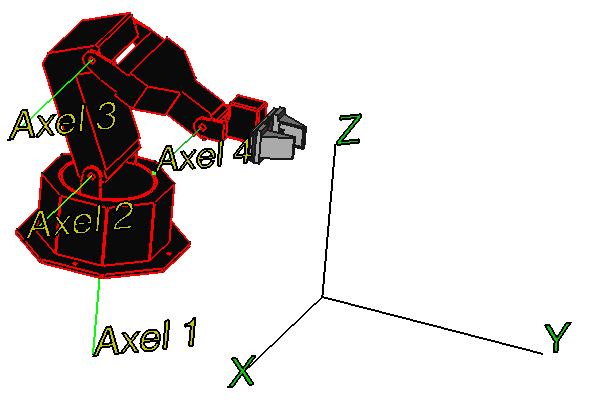
\includegraphics[scale=0.4]{robotaxis}}
\caption{\todo{Kaption}}
\end{figure}